\chapter{Mathematical Background}
\label{MathBack}

In order to comprehend the mathematical principles underlying the encryption algorithms described in this thesis, it is first necessary to grasp a few fundamental concepts. However, it is assumed that the reader has a basic familiarity with linear algebra and polynomial calculus.

\section{Lattice}

% Based on \cite{LatticeTutorial}.

All of the algorithms discussed in this thesis are based on lattices, which is why we will briefly focus on them in more detail. In general, lattices behave like any other vector space, but they only consist of discrete vectors. This means that the vectors only contain integers and not real numbers as in a vector space.

Let $\textbf{B} = \{\textbf{b}_1, \textbf{b}_2, \ldots, \textbf{b}_m\}$ be a set of linearly independent vectors of $\mathbb{R}^n$. The lattice $\textit{L}$ generated by $\textbf{B}$ is the set of integer linear combinations of $\textbf{B}$. $\textbf{B}$ is called the basis of the lattice $\textit{L}$. That is,
$$L(\textbf{B}) = \{a_1\textbf{b}_1 + \ldots + a_m\textbf{b}_m | a_1, \ldots, a_m \in \mathbb{Z}  \} \subset \mathbb{R}^n$$


Using a matrix $\textbf{B}$, which contains the basis vectors as column vectors, we can generate $\textit{L}$ equivalently.

$$L(\textbf{B}) = \{\textbf{B}\cdot\textbf{x} | \textbf{x} \in \mathbb{Z}^m  \} \subset \mathbb{R}^n$$

As in this definition, the integer $n$ is the \textbf{dimension} of the lattice and $m$ is its \textbf{rank}. If $m = n$, then $\textit{L}$ is a \textbf{full-rank} lattice, which is the usual case in this thesis. 

An example of a lattice based on a basis $\textbf{B}$ and all the points that can be created with it, also called the \textbf{span}, can be seen in the figure \ref{fig:latticeGrid}.

\begin{figure}[ht]
  \centering
  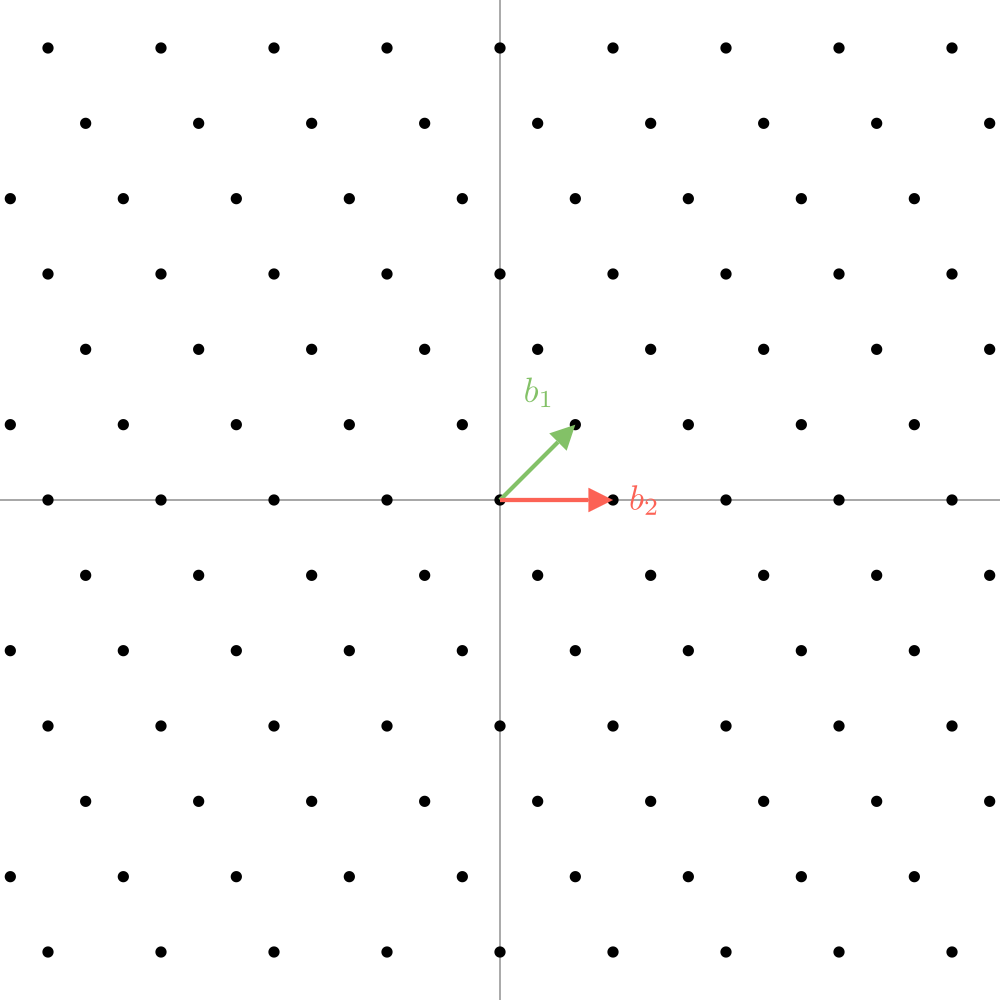
\includegraphics[scale=0.2]{images/LatticeGrid.png}
  \caption[Span of an Lattice]{The span of an two-dimensional lattice with basis  $B = \{b_1, b_2\}$.}
  \label{fig:latticeGrid}
\end{figure}

% Nur dann benötigt wenn ich genauer auf die Funktionsweise von LWE eingehen will
% \section{Shortest Vector \& Closest Vector Problem}


\section{Integer \& Polynomial Rings with modulus}
This section is based on the Book \textit{Algebra} by \textit{D. Plaumann}\cite{Algebra}.

\subsection*{Rings}
A ring is a set $R$ on which addition ($+$) and multiplication ($\cdot$) can be performed and results in a new Element, which is also part of the set R.
\begin{center}
  $ +: R+R\rightarrow R$ (Addition) and $\cdot: R \cdot R \rightarrow R$ (Multiplication)
\end{center}

These calculations need to fulfill the following conditions:
\begin{description}
  \item for addition: $R$ is an abelian group
        \begin{itemize}
          \item Associative property: $(a+b)+b = a+(b+c) | a,b,c \in R$
          \item Commutative property: $a+b = b+a | a,b \in R$
          \item Additive identity: There exists and element $0 \in R$ so that $a+0 = a | a \in R$
          \item Additive inverse: For each $a \in R$ there is an $-a \in R$ so that $a+(-a)=0$
        \end{itemize}
  \item for multiplication: R is an monoid
        \begin{itemize}
          \item Associative property: $(a\cdot b) \cdot b = a \cdot(b\cdot c) | a,b,c \in R$
          \item Multiplicative identity: There exists and element $1 \in R$ so that $a \cdot 1 = 1 \cdot a = a | a \in R$
        \end{itemize}
  \item Addition and Multiplication are distributive
        \begin{itemize}
          \item  $a\cdot (b + c) = a\cdot b + a\cdot c | a,b,c \in R$
          \item  $(a + b) \cdot c= a\cdot c + b\cdot c | a,b,c \in R$
        \end{itemize}
\end{description}

A ring is also called commutative if the multiplication is also commutative. For example, the ring over all integers $\mathbb{Z}$ is a commutative ring.

\subsection*{Modular arithmetic on Rings}

Congruence arithmetic, or modular arithmetic, is the term used to describe arithmetic with remainders when dividing integers. In everyday life, this is mainly encountered in connection with clocks. After 60 minutes, the minute hand returns to the same position as before. 

More generally, this can be described as $a \equiv b \mod q | a,b \in \mathbb{Z}, q \in \mathbb{N}$, where $q$ is the module by which $a$ and $b$ are divided until the remainder of both is less than $q$. If $a$ and $b$ are then equal, they are congruent. Or in a more mathematical expression: If there is a $k$, such as $a-b = k\cdot q$, then $a$ and $b$ are congruent.

An congruence relation with module $q$ on the set $\mathbb{Z}$, has the following properties:
% Based on \cite{Algebra} Seite 13.
$k,q \in \mathbb{N}$ and $a, a', b, b', c \in \mathbb{Z}$
\begin{enumerate}
  \item $a \equiv a \mod q$ (Reflexivity)
  \item $a \equiv b \mod q$ \textbf{if} $b \equiv a \mod q$ (Symmetry)
  \item \textbf{If} $a \equiv b \mod q$ \textbf{and} $b \equiv c \mod q$ \textbf{then} $a \equiv c \mod q$ (Transitivity)
  \item \textbf{If} $a \equiv a' \mod q$ \textbf{and} $b \equiv b' \mod q$ \textbf{then} $a+b \equiv a'+b' \mod q$
  \item \textbf{If} $a \equiv a' \mod q$ \textbf{and} $b \equiv b' \mod q$ \textbf{then} $a\cdot b \equiv a'\cdot b' \mod q$
  \item If $c$ and $q$ are coprime and $c \cdot a \equiv c \cdot b \mod q$ \textbf{then} $a \equiv b \mod q$
  \item \textbf{If} $a \equiv b \mod k\cdot q$ \textbf{then} $a \equiv b \mod q$
\end{enumerate}

The congruence class is the set of all numbers for an integer $a \in \mathbb{Z}$ modulus $q$ that produce the same remainder. It is defined as
$$[a]_q = \{b \in \mathbb{Z} | a \equiv b \mod q\}$$

It follows that two numbers are congruent if both congruence classes are equal:

$$a \equiv b \mod q \Leftrightarrow [a]_q = [b]_q$$

With this we can create a set of all congruence classes modulo $q$:
$$\mathbb{Z}_q = \mathbb{Z}/q = \mathbb{Z} \mod q = \{[a]_q | a = 0, 1, \cdots, q-1 \}$$.

For example, $Z_3 = \{[0]_3, [1]_3, [2]_3\}$. With addition and multiplication it is possible to create a commutative ring from $\mathbb{Z}_q$.
\begin{center}
  $[a]_q + [b]_q = [a+b]_q$ (addition) and $[a]_q \cdot [b]_q = [a\cdot b]_q$ (multiplication)
\end{center}

This allows to create finite rings $\mathbb{Z}_q$ for every natural number $q$ with $q$ elements in each ring and to perform calculations inside these rings. For example, an ring with $n=60$ can be created, which represents the minutes in every hour. If the minute hand shows now $48$ and we want to know where it is after $3$ times $13$ minutes, we can calculate it like:
$$[48]_{60} + [3]_{60}\cdot [13]_{60} = [48+3\cdot 13]_{60} = [87]_{60} = [27]_{60}$$

\subsection*{Polynomial Rings}

A polynomial with coefficients in a ring $R$ is expressed as 
$$f = a_0+ a_1x+\cdots+ a_{n-1}x^{d-1}+a_dx^d | a_0, \cdots, a_d \in R$$

The variable $d$ defines the degree $\deg(f)$ of the polynomial, which is the largest exponent in a polynomial.

They can be added and multiplied like any other polynomial. Such a polynomial ring with one variable $x$ and its coefficients in $R$ is written as $R[x]$. This is a generalization of the rings we had before, because $R$ is a subset of $R[x]$ ($R \subset R[x]$), since $R$ is a polynomial with $\deg(0)$: $R = R[x] := a\cdot x^0 = a$.

Such a polynomial ring can also be defined over a finite ring, so that each coefficient is part of that finite ring. This is written as $R_q = \mathbb{Z}_q[x]$. The coefficients follow the same rules for addition and multiplication as described above. The following example takes place in the ring $R_5 = \mathbb{Z}_5[x]$ and $f, g \in R_5$ with $f=1+2x+3x^2$ and $g=4+2x$:

\begin{align*}
  f\cdot 4 & = (1+2x+3x^2) * 4                                 \\
           & = [4]_5+[8]_5x+[12]_5x^2                          \\
           & = 4+3x+2x^2                                       \\
  f+g      & = (1+2x+3x^2)+(4+2x)                              \\
           & = [5]_5+[4]_5x+[3]_5x^2                           \\
           & = 4x+3x^2                                         \\
  f\cdot g & = (1+2x+3x^2)\cdot(4+2x)                          \\ 
           & = [4]_5+[2]_5x+[8]_5x+[4]_5x^2+[12]_5x^2+[6]_5x^3 \\
           & = [4]_5+[10]_5x+[16]_5x^2+[6]_5x^3                \\
           & = 4+0x+1x^2+1x^3                                  \\
\end{align*}

As with any polynomial multiplication, the degree can increase as you multiply two polynomials, leading to increasingly larger polynomials with each multiplication. Since the modulo operation creates a finite ring, we can also create a modulo operation that creates a finite ring over a polynomial where the degree stays the same or is less than some upper bound. For this we have a ring $R$ and $f, g, q, r \in R[x], g\neq 0$, where $f$ is a polynomial, $g$ is the modulus, and $r$ is the remainder:
\begin{center}
  $f = g\cdot q + r $ and $\deg(r)<\deg(g)$.
\end{center}

After this calculation, $r$ will be the remainder of $f$ with a degree smaller than that of $g$, which will be used for further calculations. With this, we can now define polynomial rings that have a module to generate finite coefficients and a polynomial function to generate finite degree. This is written as 
$$R_q = \mathbb{Z}_q[x]/f(x)$$


In this thesis the modulus function $f(x)$ will be an cyclotomic polynomial with shape $x^d+1$. To generate these $d$ needs to be a power of two ($2,4,8, \cdots$). These polynomials are used as they simplify the calculation of the remainder, because the polynomial division can be simplified to simpler addition and subtraction. When doing a polynomial division, one can simply subtract $d$ from the exponent and invert the coefficient if the exponent is greater than or equal to $d$. This must be repeated until the largest exponent is less than $d$. For example, $f \in \mathbb{Z}_5[x]/(x^3+1)$

\begin{align*}
  f & = 3+4x^2+2x^3+x^5+3x^6 & \mod (x^3+1) \\
    & = 3+4x^2-2-x^2-3x^3    & \mod (x^3+1) \\
    & = 3+4x^2-2-x^2+3                      \\
    & = 4+3x^2
\end{align*}

\section{Polynomial Ring arithmetic using Vectors \& Matrices}
\label{sec:PolyMulMath}

When calculating with polynomials, this can also be broken down into vector and matrix calculations. As we will see, this has advantages in performance, but also makes it easier to represent the polynomials when programming, as they can be handled as arrays of numbers. To create to generate vectors from polynomials, each polynomial is separated into two vectors, the coefficient vector and the variable vector.
$$
  f(x) = a_0+ a_1x+\cdots+ a_{d-1}x^{d-1}+a_dx^d =
  \begin{bmatrix}a_0\\a_1\\ \vdots \\a_{d-1}\\a_d \end{bmatrix}
  \cdot
  \begin{bmatrix}1 & x & \cdots & x^{d-1} &  x^d \end{bmatrix}
$$

The variable vector will always have the same shape as the coefficient vector. Because of the ring properties, the variable vector can always be factored out, since all polynomials have the same one in common. For this reason, only the coefficient vector will be written out in this thesis, to simplify the formulars.

When doing addition with such vectors, we just need to make sure that the vectors have the same length, which means that the polynomials must have the same degree. If this is not the case, we can fill the shorter vector with 0 so that they have the same degree. As our polynomials are always defined in a commutative  ring, the associative, commutative and distributive properties apply. So addition would look like the following:

\begin{align*}
  f(x) + g(x) & = {
  (a_0+ a_1x+\cdots+ a_{d-1}x^{d-1}+a_dx^d)+
  (b_0+ b_1x+\cdots+ b_{d-1}x^{d-1}+b_dx^d)
  }                  \\
              & = {
  \begin{bmatrix}
    a_0     \\
    a_1     \\
    \vdots  \\
    a_{d-1} \\
    a_d
  \end{bmatrix} + 
  \begin{bmatrix}
    b_0     \\
    b_1     \\
    \vdots  \\
    b_{d-1} \\
    b_d     \\
  \end{bmatrix} }     = {
  \begin{bmatrix}
    a_0     +     b_0   \\
    a_1     +  b_1      \\
    \vdots              \\
    a_{d-1} +   b_{d-1} \\
    a_d +   b_d         \\
  \end{bmatrix}
  }                  \\
\end{align*}

The process of multiplication is somewhat more complex, as the degree typically increases when two polynomials are multiplied together. As previously demonstrated, this is not the case when calculations are conducted within a polynomial ring. Accordingly, the polynomial ring $R_n = \mathbb{Z}_q/(x^d+1)$ ensures that the degree of the polynomial will never exceed $d$. Consequently, even when performing multiplication, the degree will remain less than $d$. In order to perform polynomial multiplication as a vector operation, convolutions serve as an effective tool. These can be employed for a variety of polynomial multiplications, with a particular prevalence in the Fast Fourier Transform algorithm. In this context, they are employed to reduce the polynomial-polynomial multiplication with subsequent polynomial division for the modulus into a representation of matrix-vector multiplication. The objective is to construct a matrix that encodes not only the polynomial-polynomial multiplication but also the subsequent division. To achieve this, it is essential to utilise the cyclotomic polynomial as a module and ensuring that the two polynomials are part of the same ring. This can be expressed as $f, g \in \mathbb{Z}_q/(x^d+1)$. In order to construct the calculation, one of the vectors must be transformed into a circulant matrix, where the diagonal and the lower triangle are positive and the upper triangle (without diagonal) is negative. This matrix is then multiplied by the other coefficient vector, resulting in the output coefficient vector. This new coefficient vector is identical to the result of the aforementioned polynomial multiplication with subsequent division. The general case is illustrated below:

$$
  f(x) \cdot g(x)
  =
  \begin{bmatrix}
    a_0     & -a_{d}  & -a_{d-1} & \cdots & -a_2   & -a_1   \\
    a_1     & a_0     & -a_{d}   & \cdots & -a_3   & -a_2   \\
    a_2     & a_1     & a_0      & \cdots & -a_4   & -a_3   \\
    \vdots  & \vdots  & \vdots   & \ddots & \vdots & \vdots \\
    a_{d-1} & a_{d-2} & a_{n-3}  & \cdots & a_0    & -a_{d} \\
    a_{d}   & a_{d-1} & a_{d-2}  & \cdots & a_1    & a_0    \\
  \end{bmatrix}
  \cdot
  \begin{bmatrix}
    b_0     \\
    b_1     \\
    b_2     \\
    \vdots  \\
    b_{d-2} \\
    b_{d-1}
  \end{bmatrix}
  = 
  \begin{bmatrix}
    c_0     \\
    c_1     \\
    c_2     \\
    \vdots  \\
    c_{d-2} \\
    c_{d-1}
  \end{bmatrix}
$$

The following examples will show this for two polynomials $f, g \in \mathbb{Z}_q/(x^3+1)$ with $f(x) = 3x^2+4x+1$ and $g(x) = x^2+6x+3$, using a normal polynomial multiplication and subsequent modulo, and the same with an single matrix-vector multiplication.

\begin{align*}
  f(x)\cdot g(x) & = (1+4x+3x^2) \cdot (3+6x+x^2)                & \mod x^3+1 \\
                 & = 3+6x+x^2 + 12x+24x^2+4x^3 + 9x^2+18x^3+3x^4 & \mod x^3+1 \\
                 & = 3+18x+34x^2+22x^3+3x^4                      & \mod x^3+1 \\
                 & = 3+18x+34x^2-22-3x                           &            \\
                 & = -19+15x+34x^2                               &            \\
  f(x)\cdot g(x) & = (1+4x+3x^2) \cdot (3+6x+x^2)                & \mod x^3+1 \\
                 & = {
  \begin{bmatrix}
    1 & -3 & -4 \\
    4 & 1  & -3 \\
    3 & 4  & 1  \\
  \end{bmatrix}
  \cdot 
  \begin{bmatrix}
    3 \\
    6 \\
    1 \\
  \end{bmatrix} }                                                             \\
                 & = {
  3 \cdot \begin{bmatrix}
            1 \\
            4 \\
            3 \\
          \end{bmatrix}
  + 6 \cdot   \begin{bmatrix}
                -3 \\
                1  \\
                4  \\
              \end{bmatrix}
  + 1 \cdot   \begin{bmatrix}
                -4 \\
                -3 \\
                1  \\
              \end{bmatrix}
  }                                                                           \\
                 & = \begin{bmatrix}
                       -19 \\
                       15  \\
                       34  \\
                     \end{bmatrix}                                          \\
                 & = -19+15x+34x^2                                            \\                     
\end{align*}

After these calculations the modulo operation could be applied on the coefficients either in the polynomial or in the vector, to generate the finite coefficient ring.

\section{Multidimensional Rings}

Rings can be not only in one dimension, but also in higher dimensions. This is written, as usual, with the dimensions as exponents in the ring. So a $m \times n$ ring matrix with modulus $q$ would be written as $\mathbb{Z}^{m\times n}_q$.

The same can be done with finite polynomial rings. To make it easier, we will first define the ring $R = \mathbb{Z}_q[x]/(x^d+1)$ and based on this ring we will define the form of a variable like $\textbf{A} \in R^{m\times n}$, which would result in a $m \times n$ matrix where all values are elements of the finite polynomial ring $R$.

In higher dimensions, calculations are carried out in accordance with the standard mathematical rules. The aforementioned method is employed for the purpose of multiplying higher-dimensional finite polynomial rings. This transformation entails the conversion of each polynomial into a vector, or a matrix in the case of a multiplication. The process results in the generation of matrices of matrices and vectors of matrices, which can be regarded as larger matrices due to the commutative law. Consequently, the dimensions of matrices and vectors are augmented by the polynomial degree, $d$. For a more comprehensive illustration of this concept, please refer to Appendix \ref{app:ExampleMultiRingCalc}.